% Chapter 4

\chapter{Experimental Setup} % Write in your own chapter title
\label{Chapter4}
\lhead{Chapter 4. \emph{Experimental Setup}} % Write in your own chapter title to set the page header


\section{The Neutron Interferometer}
The neutron interferometer that this thesis refers to is located at the Neutron Interferometry and Optics facility (NIOF) at the National Institute of Standards and Technology (NIST) in Gaithersburg, MD. 
\subsection{NIST}
\subsection{Reactor}
NIST operates a 20MW split-core research reactor. Neutrons of approximate energy $1 MeV$ are emitted during $^{235}U$ fission and then thermalized using heavy water ($D_2O$) as a moderator. This brings the neutrons to room temperature as discussed in (\ref{sec:thermal}). At the reactor core the peak thermal neutron flux is $4\times 10^{14} neutrons/cm^2$. The reactor is operated on a seven week cycle during which it is operated at full power for 38 days and then followed by 11 days of refuelling and maintenance operations. 

As the longer wavelength of cold neutrons ($\lambda>1.8\AA$ and $E<25meV$) is often desired for condensed matter study there is a cold moderator installed next to the core. The thermal neutrons scatter with liquid hydrogen at $20K$ and exit with a Maxwellian distribution of characteristic temperature of $34K$. 

There are eight thermal neutron ports available for lab use. The neutrons are transported to the instruments in the NCNR hall using neutron guides. The neutron interferometer facility is located on the NG7 guide shown in figure (\ref{fig:guides}). The guides are of a rectangular cross-section and are produced by gluing together meter long sections of $100nm$ thick $^{58}Ni$ optically-flat borated glass plates. $^{58}Ni$ is used due to its large neutron reflective potential. 
$$V = \frac{2\pi*\hbar^2}{m}\rho=\frac{2\pi\hbar^2}{m}\frac{1}{V}\sum\limits_{i} b = 335neV$$



\subsection{Motors and Actuators}
The neutron interferometry lab uses a variety of motors and actuators that allow experimental parameters to be controlled over the wire. Depending on the device communication is achieved via analog or digital protocols.
\subsubsection{Newport 301}

The Newport ESP301 is a three axis motion controller and driver.\cite{esp301manual} It can drive both DC servo motors and 2-phase stepper motors at up to 3 amps. It has a 1000x micro-step resolution per axis which allows very fine grained control of movements which is necessary for precision measurements. The Newport ESP 301 is primarily used to drive servo motors that orient the phase flag in the neutron interferometer. Precise angular control is a must as this is one of the primary experimental parameter. The device can also be used to control the interferometry stage to orient it. 

The Newport device utilizes encoder feedback built into servos to obtain precise positional feedback. While most Newport brand motors will automatically supply their configuration information, the equipment at NIST is not necessarily compatible in such a way. Therefore advanced configuration must be supplied by the device programmer. 

The ESP301 is controllable via a fairly extensive language of approximately 100 commands, a large portion of which are necessary for the device to be controlled successfully. Valid configuration information must be supplied. Commands are transmitted via ASCII characters according to the selected protocol. Supported protocols are serial RS232C, USB and IEEE488 with delays of $7-30ms$,$3.5ms$ and $1ms$ respectively.

\begin{figure}[ht!]
\centering
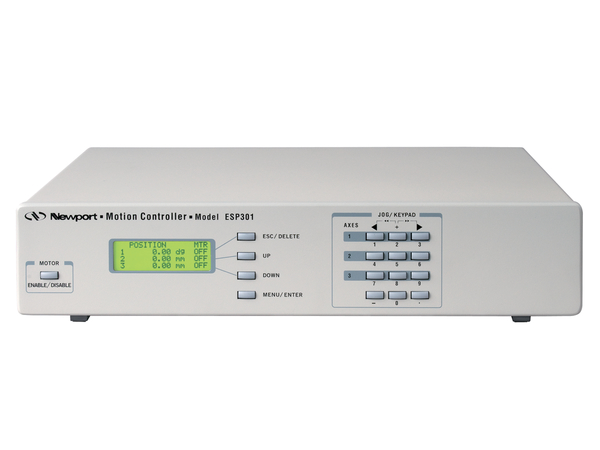
\includegraphics[scale=0.5]{Figures/esp301.jpg}
\caption{Newport ESP301 three axis motion controller}
\label{fig:esp301}
\end{figure}
\subsubsection{Kepco Power Supply}
Kepco series ATE power supplies are used to control a variety of devices in the interferometry lab. Specifically the 15-6M and 36-15M models are used and are rack mounted. The models are rated at ($0$-$15V$,$0$-$6A$,$50W$) and ($0$-$36V$,$0$-$15A$,$500W$) respectively.\cite{kepco} The models are controllable via an analog input line that sets the supply output as a linear function of the input from $0$-$10V$. Additionally there is a crowbar voltage controller which allows a maximum voltage to be set in a similar manner. The Kepco supplies are controllable via DACs which are managed via a LabJack. 
\subsubsection{LabJack}
The LabJack is a low cost measurement and automation platform. Specifically NIST will use the U3-LV variant. The U3-LV provides up to 16 analog inputs, 2 analog outputs and up to 20 digital I/O pins. The analog inputs accept voltages from $0$-$3.6V$ and the onboard DACs outputs from $0$-$5V$. The LabJack devices are easily controlled via a Python API. 

In Addition to the LabJack the LJTick-DACs, a DAC made to be digitally controlled by LabJack devices are used to provide control inputs to devices such as the Kepco power supplies. The LJTick-DAC outputs $\pm10V$  controllable by the LabJack pins in which it is inserted too. Each LJTick-DAC provides two DACs. 
\begin{figure}[ht!]
\centering
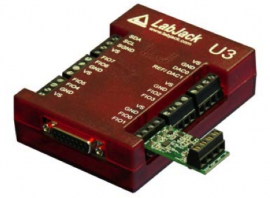
\includegraphics[scale=0.5]{Figures/labjack.png}
\caption{Labjack U3 with LJTick-DAC}
\label{fig:labjack}
\end{figure}
\subsection{Sensors}
As the likelihood method for the contrast measurement is a function of the temperature and humidity of the interferometer chamber, a variety of measurements must be taken using many different sensors.
\subsubsection{EI1050 Temperature and Humidity Probe}
The EI1050 is a digital temperature and humidity probe produced by LabJack. While its protocol is open source, it has been designed to be used with a LabJack device and sample code has been provided. The device is not especially accurate as it is rated at $\pm0.5^{\circ}$ and $\pm3.5\%$ humidity at ranges from $-40$-$120C$ and $0$-$100\%$ humidity. It is still useful to provide a quick and easy measurement. 
\subsubsection{Stanford Research Systems CTC100 Temperature Controller}
The SRS CTC100 is a cryogenic temperature controller. It provides four sensor inputs, four analog outputs and six feedback control loops. Temperature readings are made by thermistor sensors and heating is provided by resistive heaters. The device is programmable using USB, Ethernet and either GPIB or RS-232 inputs. Commands are provided via ASCII commands.  
The thermistor temperature readings are very accurate with an accuracy of $\pm0.25\Omega$ for a $300\Omega$ thermistor. The CTC100 automatically supplies the mean and standard deviation of sampled temperatures. 
\begin{figure}[ht!]
\centering
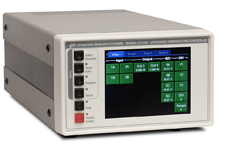
\includegraphics[scale=1.0]{Figures/ctc100.jpg}
\caption{Stanford Research Systems CTC100: Cryogenic Temperature Controller}
\label{fig:ctc100}
\end{figure}
\section{NI-Engine}
The current system at the NIST interferometry lab uses an Excel spreadsheet connected via ActiveX to closed source controller code. This system only controls the bare minimum of experimental hardware and is very inflexible. The system is not easily extensible and the software design principles are very poor. As the contrast improvement experiment requires many different sensor inputs and system controllability for many different measurement cases, it would have been a tremendous task to implement into the current system. 

Ni-Engine attempts to solve the problems of the previous system for the proposed experiment and future lab researchers. NI-Engine is an experimental neutron interferometry control system programmed in Python using open source libraries and software design principles.
\subsection{Design Requirements}
\label{sec:requirements}
The core design requirement of NI-Engine are to be a complete, easy to use neutron interferometry experimental control system. In order fulfil this core requirement the software had to fulfil these requirements: 
\begin{itemize}
  \item Be able to communicate with and control a large range of hardware in a manner that allows powerful functionality while hiding the inherent complexity. 
  \item Handle experimental setup and configuration via configuration files such that an experimental setup is easily repeatable given an identical configuration. 
  \item Handle the collection and storage of experimental data. Experimental data will be large, possible into the $10+GB$ range. Should allow for multiple identical experiments to be performed sequentially.
  \item Execution of software functionality must be fast and allow for experiment running times to be dominated by hardware measurement and control, rather than software running time. 
  \item Software must be able to run for long periods of time with consistent memory requirements.
  \item Data should be collected and stored with units available to avoid confusion.  
  \item Should be modular. Outside researchers should be able to modify software to their own requirements. ie. addition of new hardware, file formats, data types. 
  \item Software must have extensive documentation and example code. Researchers should be able to utilize without extensive outside help.  
\end{itemize}
These design requirements had to be taken into account when designing and programming Ni-Engine
\subsection{Language and Software Library Choices}
\subsubsection{Language}
Given the design requirements outlined in (\ref{sec:requirements}) it is clear that the system required is quite extensive. Python\cite{python} was selected as the development language for Ni-Engine. Python was selected for a variety of reasons including 
\begin{itemize}
\item Python is very easy to learn and use. Its syntax style allows newcomers the ability to quickly write code, while still allowing experts powerful expressibility. 
\item Python's code is extremely legible and the nature of its syntax naturally generates readable code. 
\item Python has many powerful libraries available that when used allow rapid development of complex software without the complexity of rolling ones own solution. 
\item Python has a large and help community. 
\item It is very easy to interface with C based code if performance is desired. 
\item Python is object oriented which when used correctly allows simple creation of modular and extensible software. 
\item Python is dynamically typed and evaluated which allows rapid iteration and ease of use at the cost of performance and security. 
\end{itemize}
While the use of python does come at some costs, namely memory and CPU performance, on a whole the choice of language provided enormous benefits.

\subsubsection{Software Libraries}
Due to the nature of an experimental system composed of heterogeneous hardware there is a lot of complexity in communicating with hardware over different communication channels. To overcome this challenge the library  InstrumentKit\cite{instrumentKit} was used. InstrumentKit allows identical commands to be sent over a variety of different communication channels at a high level of abstraction. It was a much more simple matter to contribute communication code for necessary sensors and hardware to InstrumentKit and then just utilize the library. As Ni-Engine must handle large volumes of data and manipulate this data, Numpy\cite{numpy} was used for its efficent handling of arrays in Python and the variety of methods it provides. To store this data the first file format to be implemented was HDF5\cite{hdf5}, which is a version of the Hierarchical Data Format. HDF5 was designed for the storage of large amounts of numerical data. Additionally, it provides an easily navigable hierarchical file system. Creation and manipulation of HDF5 files was facilitated by the memory efficient H5py\cite{h5py} library for Python. Configuration data is in the YAML\cite{yaml} format and is manipulated using PyYaml\cite{pyyaml}. As the main goal of the system is to handle experimental data that is often associated with physical units of measurement Python units\cite{units} was used. Units allows the wrapping of Python data types and Numpy arrays in physical units, and performs the necessary unit operations when performing operations between data types of units. 

As extensive documentation is a core design requirement of Ni-Engine, it was essential that a documentation generation library be used throughout development. Sphinx\cite{sphinx}, the De facto Python standard for documentation pulls in-code comments and generates relational documentation in a variety of formats including html and pdf formats. 
\subsection{System Architecture}
Ni-Engine is split into several major components controlled by the main NiEngine object. Major components are the configuration, hardware, controllers, sensors and storage sections. 
\subsubsection{Design Patterns}
Due to the complexity of Ni-Engine it was necessary to use object oriented design patterns. The main NiEngine class controls the execution and control flow of the experimental system. During execution of an experiment all commands initially must go through the NiEngine class. Ni-Engine follows a chain of responsibility pattern and has a strict hierarchy with NiEngine sitting at the top.

Ni-Engine divides the software into five separate components, each of which attempts to be as modular as possible, allowing the modification of internals without the affecting the behaviour of the system as a whole. The main sections are the configuration, hardware, controller, sensors and storage sections. The NiEngine object reads in the experimental configuration via the Configuration object and supplied file. From there, it dispatches creation of experimental software components HardwareManager, ControllerManager, SensorManager and DataHandler objects which are responsible for their self-descriptive duties.

\begin{figure}[ht!]
\centering
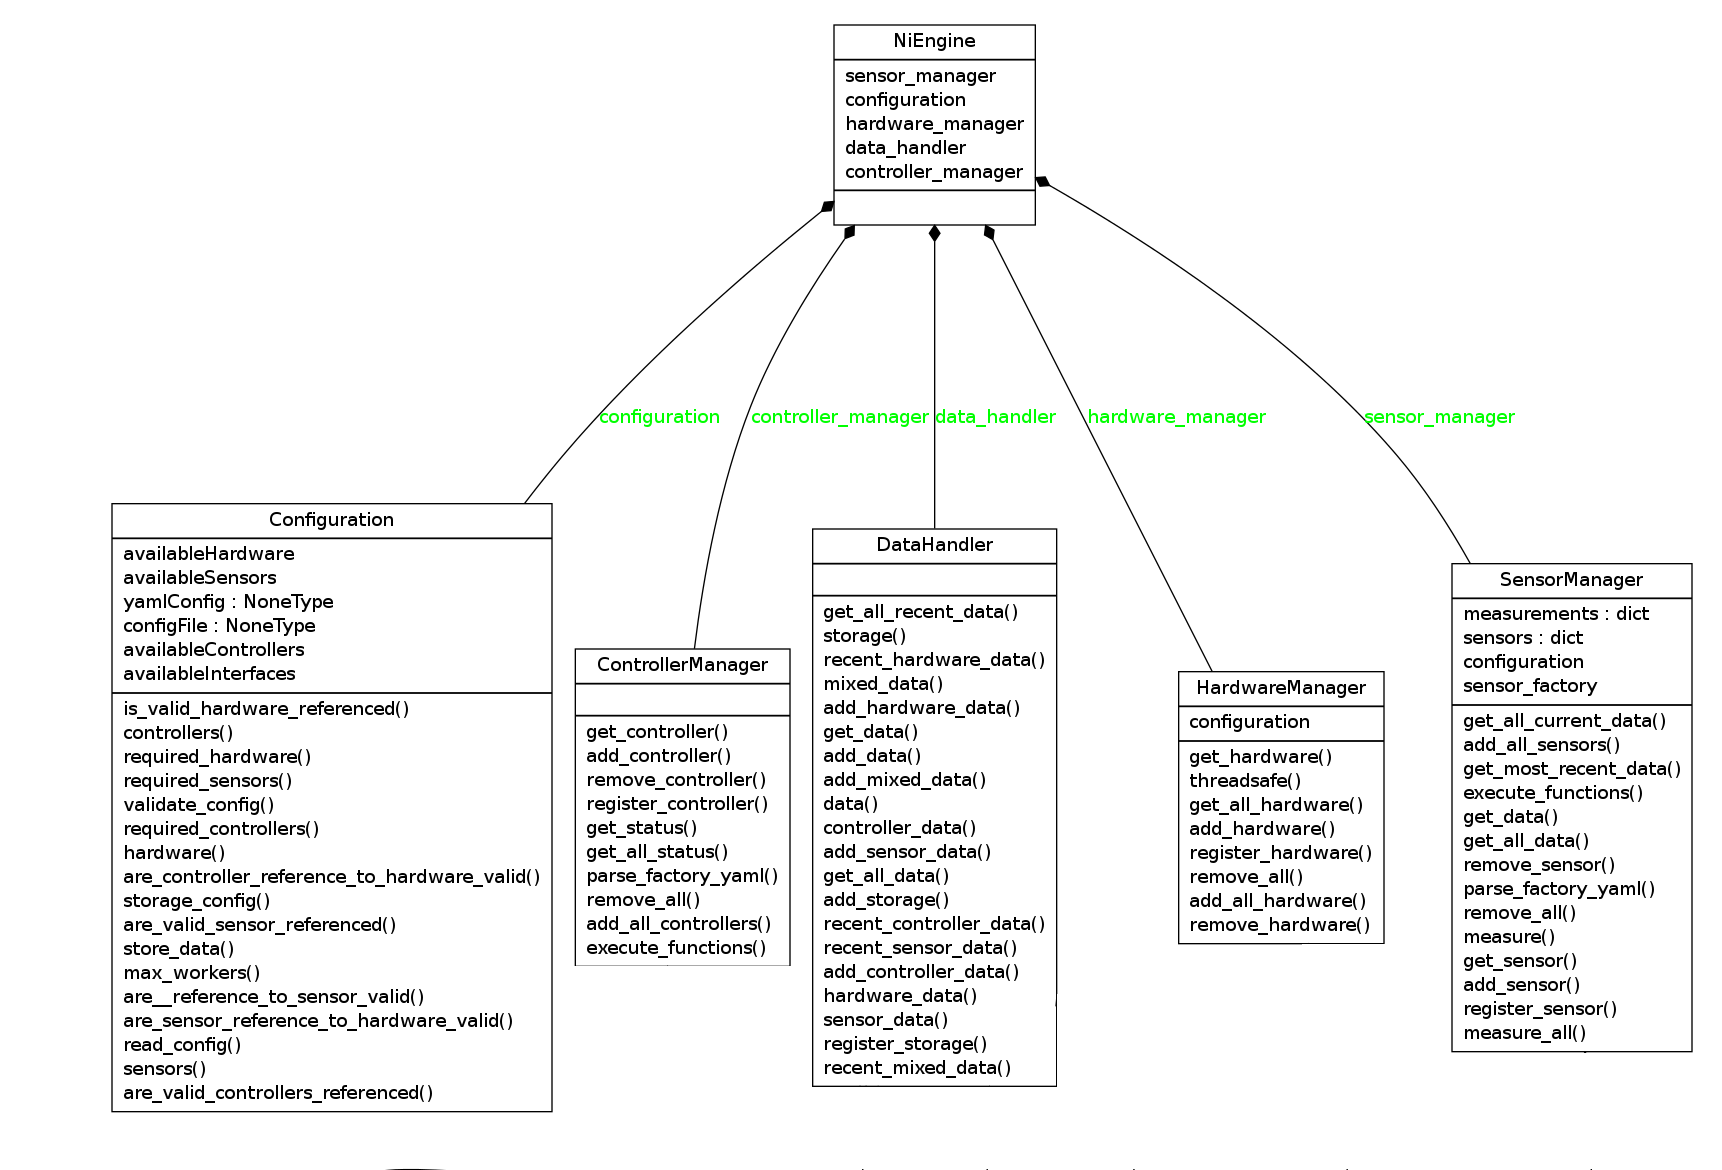
\includegraphics[width=\textwidth]{Figures/NiEngine.png}
\caption{NiEngine object control hierarchy}
\label{fig:NiEngine}
\end{figure}
\subsubsection{Configuration}
A core tenet of the design of Ni-Engine was that it has to make experiments easily scriptable and repeatable. As experimental hardware requires many different configuration values to be set, that if set incorrectly can result in disastrous consequences it is infeasible to supply configuration via the command-line or as python based configuration. Therefore configuration is provided to Ni-Engine via Yaml configuration files which allows the specification of all runtime configuration options for Ni-Engine. This allows experiments to be run with the same initial settings consistently simply by passing Ni-Engine a predefined configuration file. Configuration is made simple thanks to Yaml's hierarchical data format, which is converted into a very simple to use Python dictionary by PyYaml. 
\subsubsection{Data Storage}
Ni-Engine utilizes a storage format agnostic API. All storage communication is channelled through a DataHandler instance. At initialization time DataHandler is a passed its required configuration information as defined in the experiments configuration file. It is possible to utilize many different file formats provide a class that implements the AbstractPhysicalStorage is provided and it is registered with the main Ni-Engine class. This Builder pattern allows future extensibility and interaction, although at current time only the HDF5 file format is supported. 

In Ni-Engine all measurements reside in memory as Data objects. Data objects are interesting in that they measurement meta-information with such fields such as measurement names, measurement types and the time the measurement was taken at. All the while Data objects behave as their value data-types in code. This allows measurements to be created with essential meta-information and than to be manipulated in a normal fashion as would integers,floats, arrays and other basic data-types. 

Due to the slow nature of permanent storage devices, data to be written to storage are batched in order to limit the amount of write calls. When the buffer is filled it is flushed to the disk. A balance must be established between the amount of data stored in memory compared to how often it is written to disk. Of course any data in memory is ethereal and power failure / program crashes will cause the data to be lost. 
\begin{figure}[ht!]
\centering
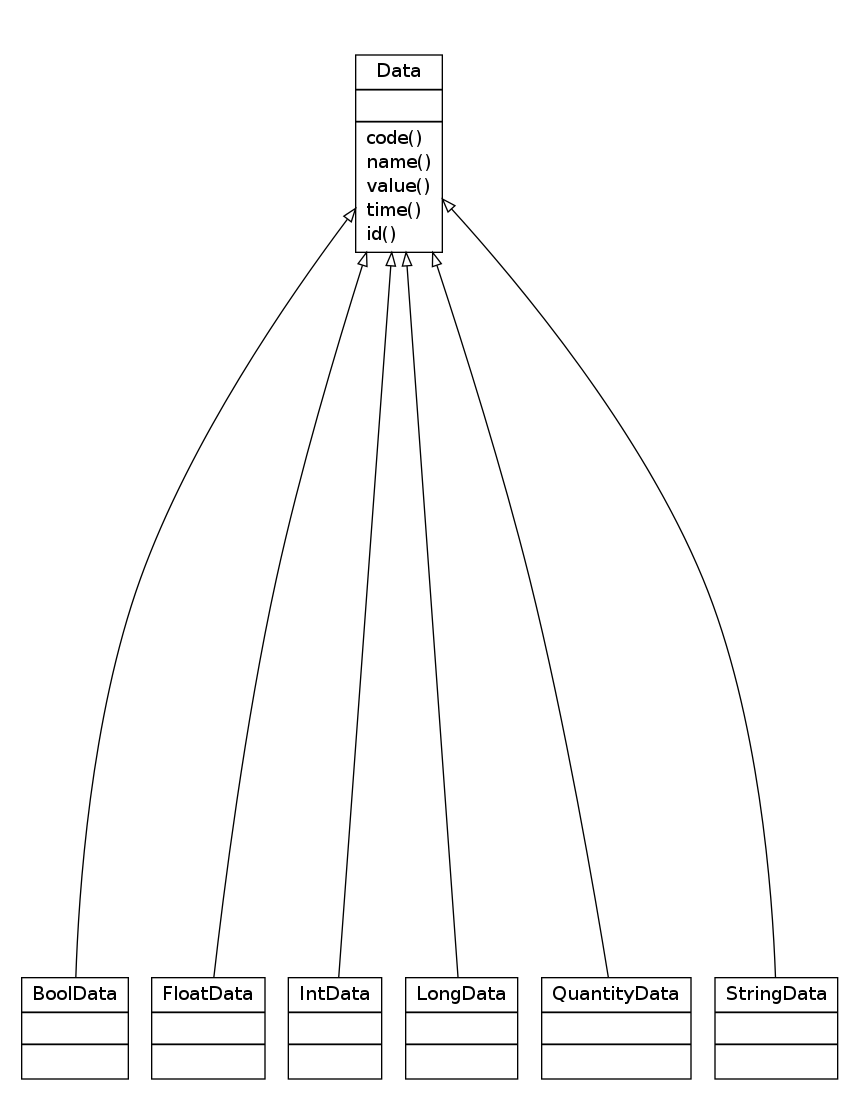
\includegraphics[width=0.6\textwidth]{Figures/datatypes.png}
\caption{Datatype measurement class}
\label{fig:datatypes}
\end{figure}
\subsubsection{Manager Objects}
In Ni-Engine all control of physical hardware is managed by the HardwareManager,ControllerManager and SensorManager objects. Managers are responsible for initialization, configuration, data acquisition and object destruction. Upon initialization these manager classes are passed configuration information that contains all necessary information for the setup and control with all experimental hardware. Each manager object creates its own singleton factory object that is responsible for constructing either the hardware, controllers or sensors for the system depending on its type. Every controller and sensor object interacts with physical hardware through hardware objects. This is to ensure that each physical device is only instantiated once and prevents race conditions. Upon creation of these experimental equipment objects they are placed under management by their respective managers. 

Measurement calls to devices are made via manager objects. Manager objects have the ability to measure individual devices or all devices at once. As differing devices have different latencies, sequential measurement can take an excessive amount of time. Therefore measurement calls are threaded to allow measurements to be performed in parallel. Of course certain sensors and controllers may utilize the same hardware and therefore race conditions can result. It is therefore important for these to devices to implement thread locking at the hardware level for these objects. After measurements are made they are passed onto the DataHandler object for storage as well as returned to the function call. 
\subsubsection{Documentation}
As the purpose of Ni-Engine is to be a general neutron interferometry experimental engine and not just to be used one time the neutron contrast experiment it is important that documentation be available for future researchers that may not have the luxury of a hands on introduction by the software designers. To increase the software ease of use

